% 指数函数(复数)
% 复数|指数函数|三角恒等式|欧拉公式|导数

%未完成
%(计划内容: 定义,复平面上的特征,是解析函数,反函数,物理上最广的应用).

\pentry{指数函数, 复数\upref{CplxNo}, 导数\upref{Der}}

\begin{figure}[ht]
\centering
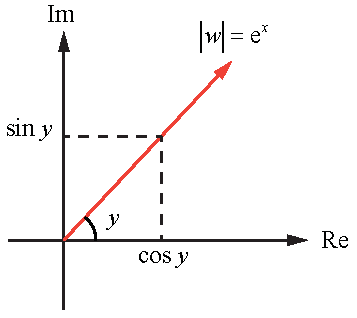
\includegraphics[width=5.7cm]{./figures/CExp_1.pdf}
\caption{复数域中的指数函数} \label{CExp_fig1}
\end{figure}

复数域中的指数函数被定义为
 \begin{equation}\label{CExp_eq1}
w = \E^z = \E^{x + \I y} = \E^x(\cos y + \I\sin y)
\end{equation}
在复平面上表示这个函数,则指数的实部 $x$ 控制因变量 $w$ 的模长, 虚部 $y$ 控制 $w$ 的幅角, 如\autoref{CExp_fig1}
 \begin{equation}
\abs{w} = \E^x \qquad \arg(w) = y
\end{equation}
当指数为纯虚数时,\autoref{CExp_eq1} 变为著名的\textbf{欧拉公式}
\begin{equation}\label{CExp_eq2}
\E^{\I x} = \cos x + \I\sin x
\end{equation}
虽然这里的 $x$ 一般是实数(物理中应用得最多的情况),但根据复数域三角函数的定义\upref{CTrig}, 对于任何复数 $z$,都有欧拉公式
\begin{equation}
\E^{\I z} = \cos z + \I\sin z
\end{equation}
将“三角函数(复数)\upref{CExp}”中的\autoref{CTrig_eq1} 和\autoref{CTrig_eq2} 代入即可证明.

根据\autoref{CExp_eq1} 的定义结合两角和公式(\autoref{TriEqv_eq1}\upref{TriEqv}), 容易证明 $\E^z$ 同样满足
\begin{equation}
\E^{z_1 + z_2} = \E^{z_1}\E^{z_2}
\end{equation}

虽然我们还没有系统地学习复变函数求导的概念, 但我们可以根据\autoref{CExp_eq2} 求出一个物理中常见的导数公式
\begin{equation}\ali{
\dv{x} \E^{\I ax} &= -a\sin(ax) + \I a\cos(ax)\\
&= \I a[\cos(ax) + \I \sin(ax)]\\
&= \I a \E^{\I ax}
}\end{equation}
进一步拓展, 令复常数 $z = a + \I b$ 得
\begin{equation}
\dv{x}\E^{z x} = \dv{x} \qty(\E^{ax}\E^{\I bx}) = (a + \I b)\E^{(a+\I b)x} = z\E^{zx}
\end{equation}
可见 $\E^z$ 的许多性质与实数域的 $\E^x$ 类似.


